\section{Introducción}
A lo largo de este informe se desarrollarán distintos circuitos con el objetivo de comprender cómo funcionan los mezcladores.\\
\\
\textbf{¿Qué es un mezclador?}\\
\indent En el campo de la electrónica, un mezclador es un circuito que procesa las señales de sus entradas para obtener a la salida una combinación de las mismas.\\
\\
\indent A lo largo de este informe se estudiará un mezclador compuesto por un único diodo.\\
Para realizar el estudio, se han diseñado distintos circuitos. El primero, consiste en un diodo (1N914) y una resistencia (de $1\ k\Omega$), los cuales se encuentran conectados en serie tal como se observa en la Figura 1. La fuente asignará al circuito una señal de voltaje constante, con valores de $0\ V$ a $1.5\ V$, variando en $0.1\ V$ para cada medición.\\
\indent El segundo circuito, que se puede observar en la Figura 2, parte de la base del anterior, pero incluyendo una fuente de ruido.\\
\\
Para el desarrollo de los circuitos de este informe se utilizó el programa LTspice.
\newpage

\section{Desarrollo y resultados}
\subsection{Marco Teórico}
Para este informe se necesitan comprender diversos elementos presentes en la electrónica. Se comenzará explicando \textbf{cómo funcionan un diodo y un mezclador simple}.\\
Un diodo es un componente electrónico de dos terminales que permite la circulación de la corriente eléctrica a través de él en un solo sentido, ​ bloqueando el paso si la corriente circula en sentido contrario, no solo sirve para la circulación de corriente eléctrica sino que este la controla y resiste. Se conoce que la corriente que circula por un diodo se define por la fórmula (1).\\
\begin{equation}
    I(V)=I_0\left(e^{\frac{q}{KT}(V_{in}-V_b}\right)
\end{equation}
donde
\begin{itemize}
    \item $I =$ Intensidad de corriente que atraviesa el diodo
    \item $V_{in} =$ Voltaje de entrada
    \item $V_b =$ Voltaje en el otro extremo del diodo
    \item $V =$ Caída de potencial en los extremos del diodo
    \item $q = $ carga del electrón (en valor absoluto) $= 1.6 \times 10^{-19}$
    \item $K = $ Constante de Boltzmann $= 1.38\times 10^{-23}$
    \item $I_0 =$ Corriente de saturación (incógnita)
    \item $T =$ Temperatura de la unión (incógnita)
\end{itemize}
Para obtener las incógnitas $I_0$ y $T$ se realizará un ajuste a los datos. Luego, en la curva $I$-$V$, el comportamiento no lineal del diodo se maximiza para el punto de máxima curvatura (mínimo radio de curvatura). Lo último se deve a que
$$X=1/R_{curvatura}$$
donde $X$ es la curvatura y $R_{curvatura}$ es el radio de curvatura.
Posteriormente se debe comprender el funcionamiento de una \textbf{Serie de Fourier}, la cual establece que toda función $\in [t_1, t_2]$ puede expresarse como una Serie de Fourier tal como indica la ecuación (2).
\begin{equation}
    f(t)=a_0+\sum\limits_{n=1}^\infty cos(n\omega_0t)+\sum\limits_{n=1}^\infty b_nsen(n\omega_0t)
\end{equation}
con
$$a_n=\frac{2}{t_2-t_1}\int\limits_{t_1}^{t_2}f(t)cos(n\omega_0t)dt$$
$$b_n=\frac{2}{t_2-t_1}\int\limits_{t_1}^{t_2}f(t)sin(n\omega_0t)dt$$
Se debe entender el concepto de que cada función expresada como Serie de Fourier es una suma infinita de senos y cosenos, donde cada $n$ indica el armónico con su frecuencia y contribución a la señal principal. Por otra parte, $a_0$ es una constante la cual en el caso de este informe vendría siendo el DC-offset.\\
Luego, se introduce el concepto de \textbf{Mezclador Simple}, el cual consiste en una resistencia y un diodo conectados en serie. En estos circuitos nos interesa el voltaje de salida, $V_{out}$, el cual se calcula con la ecuación (3)
\begin{equation}
    V_{out}=V_b-V_c
\end{equation}
Sin embargo, el circuito analizado en este informe se encuentra conectado a tiera, por lo cual $V_c=0$. Lo anterior implica que $V_{out}$ corresponde a la caída de potencial en la resistencia:
$$V_out=V_b$$
Esto se puede calcular con la Ley de Ohm, pues conocemos la corriente que pasa por el diodo, ya que al estar conectados en serie es la misma. De esta manera,
\begin{equation}
    V_{out}=RI=RI_0\left(e^{\frac{q}{KT}(V_{in}-V_{out}}\right)
\end{equation}
La expresión anterior no tiene solución analítica, por lo cual se resolverá de manera numérica.\\
Finalmente, se introduce el concepto de \textbf{detectores}, donde un medio no lineal es útil como tal, pues las frecuencias muy altas no pueden ser procesadas a gran rapidez, pero al pasarlas por un medio no lineal se pueden estudiar sus armónicos fácilmente.
Por otra parte, se obtiene el componente DC el cual indica la amplitud de la señal original.\\
En el caso desarrollado en este informe el mezclador simple corresponde a un detector que se asemeja al orden cuadrático, es decir
\begin{equation}
    V_out(t)=a_0+a_1V_{in}(t)+\frac{a_2}{2}V_{in}^2(t)+\cdots
\end{equation}
Luego, si reemplazamos $V_{in}=Acos(n\omega t)$, la expresión resultante es
$$V_out(t)=a_0+\frac{c_2A^2}{2}a_1Acos(\omega t)+\frac{a_2}{2}A^2cos(2\omega t)+\cdots$$
Donde vemos que el primer término corresponde al DC-offset, el segundo al primer armónico y el tercero al segundo armónico.
\subsection{Resultados}
Se obtuvo la Figura 1 para la curva $I$-$V$. Con el ajuste se obtuvieron los parámetros $I_0=2.671\times 10^{-9}$ [V] y $T=21-95$ K. El error cuadrático entre el ajuste y los datos fue de $8.5\times 10^{-14}$ [mA].
\begin{figure}[H]
\centering
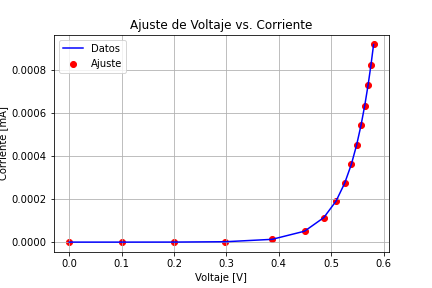
\includegraphics[scale=0.7]{img/graf1.png}
\caption{\label{fig:Grafico} Curva $I$-$V$}
\end{figure}
Luego, se calculó numéricamente la expresión (4) buscando las raíces de una función de $V_{out}$ en función de $V_{in}$. Los resultados se observan en la Figura 2.
\begin{figure}[H]
\centering
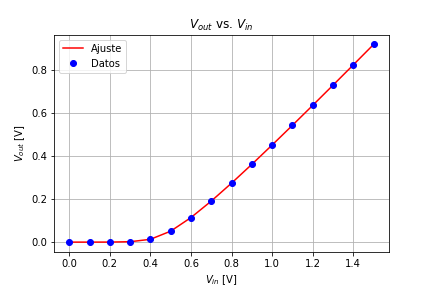
\includegraphics[scale=0.7]{img/graf2.png}
\caption{\label{fig:Grafico} $V_{out}$ en función de $V_{in}$}
\end{figure}
Luego, se han calculado las  primeras derivadas de la expresión, obteniéndose el gráfico de la Figura 3.
\begin{figure}[H]
\centering
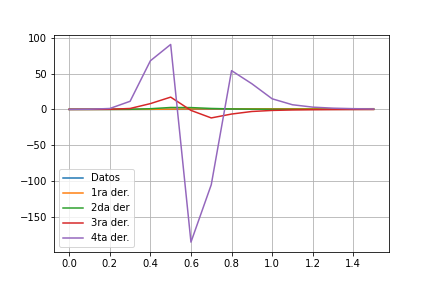
\includegraphics[scale=0.7]{img/graf3.png}
\caption{\label{fig:Grafico} Derivadas}
\end{figure}
Para calcular el punto en que se alcanza el mayor comportamiento no lineal se calcula el radio de curvatura con la expresión (6).
\begin{equation}
    R_{curvatura}=\frac{\abs{1+\left(\frac{df}{dx}\right)^2}}{\abs{\frac{d^2f}{dx^2}}}
\end{equation}
Luego, se utiliza la siguiente relación, donde $X$ es la curvatura:
$$X=\frac{1}{R_{curvatura}}$$
En el gráfico se puede observar que éste alcanza su máximo en $V_{in}=0.5$ V, con un radio de curvatura de $0.458$ y un voltaje de salida de $0.051$ [V].
\begin{figure}[H]
\centering
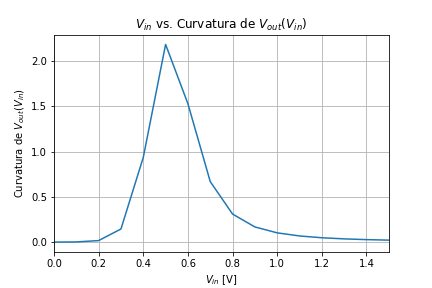
\includegraphics[scale=0.7]{img/graf4.png}
\caption{\label{fig:Grafico} Curvatura}
\end{figure}
Se nota que es equivalente el menor radio de curvatura con la mayor curvatura.\\

Para la segunda parte de este informe se cambió a una señal sinusoidal con amplitud de $0.2$ [V], frecuencia de $1$ [kHz] y un DC-offset entre $0$ y $1.5$ [V].

Se nota que todos los armónicos toman valores más altos con un $V_{in}=0.5$ [V], lo cual se muestra en la Figura 5.

\begin{figure}[H]
\centering
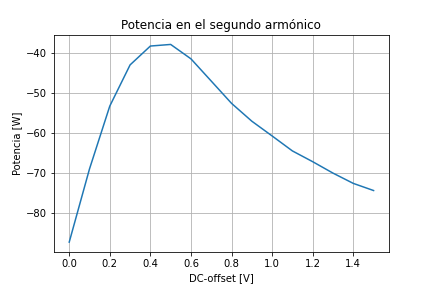
\includegraphics[scale=0.7]{img/graf5.png}
\caption{\label{fig:Grafico} Valor del segundo armónico para cada DC-offset}
\end{figure}

En la figura 7 se puede observar el espectro con un DC-offset de $0.5$ [V].
\begin{figure}[H]
\centering
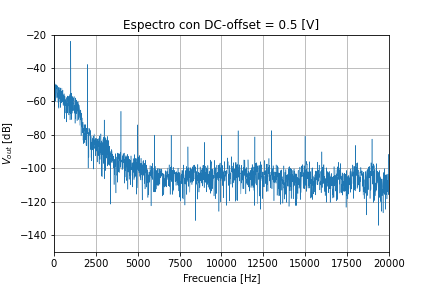
\includegraphics[scale=0.7]{img/graf6.png}
\caption{\label{fig:Grafico} Espectro con un DC-offset de $0.5$ [V}
\end{figure}

\newpage
\section{Análisis y Conclusiones}
Utilizando el software de LTspice se pudo comprobar que el ajuste de la curva $I$-$V$ coinciden con los obtenidos en dicho software, con un valor de $V_{in}=0.5$ [V].\\
\\
\indent Con respecto al segundo circuito, los valores obtenidos con LTspice no se asemejan a los obtenidos mediante la serie de Taylor, lo que se puede explicar, por ejemplo, con el ruido que se le inyectó al sistema (que hubiera ocurrido de igual manera realizando mediciones manuales) o porque la hipótesis de $V_{in}=cos(\omega t)$ no era correcta.\\
\\
\indent A modo de conclusión, se puede decir que un circuito tal como el que se utilizó puede utilizarse como detector, pues transforma la señal en una conocida, obteniendo así información de la fuente.
\newpage

\begin{sourcecode}[\label{codigo-python}]{python}
# Importamos las librerías necesarias
import numpy as np
from matplotlib import pyplot as plt
from scipy.optimize import curve_fit, bisect
from scipy.interpolate import CubicSpline
import pandas as pd
\end{sourcecode}

\begin{sourcecode}[\label{codigo-python}]{python}
V_t = np.array([0., 0.09997963, 0.19979541, 0.29818724, 0.38708739,
       0.44918412, 0.4858808 , 0.5092326 , 0.5257116 , 0.5384415 ,
       0.5484803 , 0.556853  , 0.5640389 , 0.5703152 , 0.5758803 ,
       0.5808764 ])

I = np.array([0., 2.036700e-08, 2.045907e-07, 1.813641e-06,
       1.291275e-05, 5.081596e-05, 1.141195e-04, 1.907880e-04,
       2.742902e-04, 3.617043e-04, 4.515953e-04, 5.431760e-04,
       6.359759e-04, 7.296934e-04, 8.241251e-04, 9.191271e-04])
\end{sourcecode}

\begin{sourcecode}[\label{codigo-python}]{python}
V_out = np.array([0.000000e+00, 2.036700e-05, 2.045893e-04, 1.812759e-03,
       1.291261e-02, 5.081588e-02, 1.141192e-01, 1.907674e-01,
       2.742884e-01, 3.615585e-01, 4.515197e-01, 5.431470e-01,
       6.359611e-01, 7.296848e-01, 8.241197e-01, 9.191236e-01])

V_in = np.array([0. , 0.1, 0.2, 0.3, 0.4, 0.5, 0.6, 0.7, 0.8, 0.9, 1. , 1.1, 1.2,
       1.3, 1.4, 1.5])
\end{sourcecode}

\begin{sourcecode}[\label{codigo-python}]{python}
def corriente_I(V, a, b):
    return a * (np.exp(b * V) - 1)
\end{sourcecode}

\begin{sourcecode}[\label{codigo-python}]{python}
I_fit = curve_fit(corriente_I, V_t, I)
I_teo = corriente_I(V_t, I_fit[0][0], I_fit[0][1])

print('I_0 =', I_fit[0][0], 'T =', I_fit[0][1])

suma = 0
for i in range(len(V_t)):
    suma = suma + (I_teo[i] - I[i])**2

print('El error cuadrático es de', suma/len(V_t), '[mA]')
    
plt.scatter(V_t, I_teo, label = 'Ajuste', color = 'red')
plt.plot(V_t, I, label = 'Datos', color = 'blue')
plt.title('Ajuste de Voltaje vs. Corriente')
plt.xlabel('Voltaje [V]')
plt.ylabel('Corriente [mA]')
plt.legend()
plt.grid()
plt.savefig(r"C:\Users\Usuario\Documents\Astro experimental\Informe 3\graf1.png")
plt.show()
\end{sourcecode}

\begin{sourcecode}[\label{codigo-python}]{python}
# Constantes
R = 1000
I0 = I_fit[0][0]
b = I_fit[0][1]

# voltaje de entrada y salida
V_out_fitted=np.zeros(len(V_in))

# funcion que se buscara ceros
def g(v_out):
    return R * I0 * (np.exp((V_in[i] - v_out) * b) - 1) - v_out

for i in range(len(V_in)):
    V_out_fitted[i] = bisect(g,10,-10)
    
print(V_out_fitted)
\end{sourcecode}

\begin{sourcecode}[\label{codigo-python}]{python}
plt.plot(V_in, V_out_fitted, label='Ajuste', color = 'red')
plt.plot(V_in, V_out, 'o', label='Datos', color = 'blue')
plt.title('$V_{out}$ vs. $V_{in}$')
plt.xlabel('$V_{in}$ [V]')
plt.ylabel('$V_{out}$ [V]')
plt.legend()
plt.grid()
plt.savefig(r"C:\Users\Usuario\Documents\Astro experimental\Informe 3\graf2.png")
plt.show()
\end{sourcecode}

\begin{sourcecode}[\label{codigo-python}]{python}
# pasamos a array
V_in = np.array(V_in)

# expandimos
Vind = np.append(V_in, [1.6, 1.7, 1.8])

# extrapolamos
cs = CubicSpline(V_in, V_out_fitted)

Voutd = cs(Vind)
\end{sourcecode}

\begin{sourcecode}[\label{codigo-python}]{python}
lenght = len(V_out_fitted)
d1, d2, d3, d4 = np.zeros(lenght), np.zeros(lenght), np.zeros(lenght), np.zeros(lenght)

for i in range(len(V_out_fitted)-1):
    h = 0.1 # V_in[i + 1] - V_in[i] = 0.01 siempre
    d1[i + 1]  = (V_out_fitted[i + 1] - V_out_fitted[i]) / h
    d2[i + 1] = (d1[i + 1] - d1[i]) / h
    d3[i + 1] = (d2[i + 1] - d2[i]) / h
    d4[i + 1] = (d3[i + 1] - d3[i]) / h
   
d1[0], d2[0], d3[0], d4[0]  = 1e-5 , 1e-5, 1e-5 , 1e-5

print(d4)
\end{sourcecode}

\begin{sourcecode}[\label{codigo-python}]{python}
plt.plot(V_in, V_out, label = 'Datos')
plt.plot(V_in, d1, label = '1ra der.')
plt.plot(V_in, d2, label = '2da der')
plt.plot(V_in, d3, label = '3ra der.')
plt.plot(V_in, d4, label = '4ta der.')
plt.legend()
plt.grid()
plt.savefig(r"C:\Users\Usuario\Documents\Astro experimental\Informe 3\graf3.png")
plt.show()
\end{sourcecode}

\begin{sourcecode}[\label{codigo-python}]{python}
# Insertamos la fórmula del radio
R_curv = abs((( 1 + d1 ** 2) ** (3/2)) / d2)
index = list(R_curv).index(min(R_curv))
print('El radio de curvatura mínimo es',float(R_curv[index]), 'con un voltaje de entrada de',
      float(V_in[index]),'[V] y un voltaje de salida de', float(V_out[index]), '[V]')
\end{sourcecode}

\begin{sourcecode}[\label{codigo-python}]{python}
X = 1/R_curv

plt.plot(V_in, X)
plt.title('$V_{in}$ vs. Curvatura de $V_{out}(V_{in})$')
plt.ylabel('Curvatura de $V_{out}(V_{in})$')
plt.xlabel('$V_{in}$ [V]')
plt.xlim(0,1.5)
plt.grid()
plt.savefig(r"C:\Users\Usuario\Documents\Astro experimental\Informe 3\graf4.png")
plt.show()
\end{sourcecode}

\begin{sourcecode}[\label{codigo-python}]{python}
print('Podemos ver que la curvatura máxima se encuentra en un voltaje de entrada de', V_in[list(X).index(max(X))], '[V]')
\end{sourcecode}

\begin{sourcecode}[\label{codigo-python}]{python}
P2nd = np.array([-87.346, -69.003, -53.25, -42.943,
                  -38.22, -37.82, -41.43, -47.002,
                  -52.583, -57.053, -60.750, -64.501,
                  -67.199, -70.060, -72.633, -74.421])

V_in_offset = np.array([0., .1, .2, .3, .4, .5, .6, .7, .8,
                     .9, 1, 1.1, 1.2, 1.3, 1.4, 1.5 ])
\end{sourcecode}

\begin{sourcecode}[\label{codigo-python}]{python}
plt.plot(V_in_offset, P2nd)
plt.ylabel('Potencia [W]')
plt.xlabel('DC-offset [V]')
plt.title('Potencia en el segundo armónico')
plt.grid()
plt.savefig(r"C:\Users\Usuario\Documents\Astro experimental\Informe 3\graf5.png")
plt.show()
\end{sourcecode}

\begin{sourcecode}[\label{codigo-python}]{python}
maxP = max(P2nd) # P = V \cdot I
maxDC = V_in_offset[list(P2nd).index(maxP)]

print('El valor de DC-offset donde se encuentra el',
      'máximo contenido armónico es', maxDC, '[V]',
      'con', maxP, '[W]')
\end{sourcecode}

\begin{sourcecode}[\label{codigo-python}]{python}
data2 = pd.read_table(r"C:\Users\Usuario\Downloads\circuito2clean.csv", delimiter = ',')
frequencies = data2['Freq.'] 
vouts = data2['V(out)']

plt.plot(frequencies, vouts, linewidth = 0.5)
plt.xlim(0,20000)
plt.ylim(-150,-20)
plt.xlabel('Frecuencia [Hz]')
plt.ylabel('$V_{out}$ [dB]')
plt.title('Espectro con DC-offset = 0.5 [V]')
plt.grid()
plt.savefig(r"C:\Users\Usuario\Documents\Astro experimental\Informe 3\graf6.png")
plt.show()
\end{sourcecode}

\begin{sourcecode}[\label{codigo-python}]{python}
# Calculamos la frecuencia de los armonicos

armonicos = np.array([68.34, 12.86, 0.28, 0.51])
\end{sourcecode}

\begin{sourcecode}[\label{codigo-python}]{python}
# Calculamos las derivadas en 0.5 [V]

V = V_out[5]
dV  = d1[5]
d2V = d2[5]
d3V = d3[5]
d4V = d4[5]
\end{sourcecode}

\begin{sourcecode}[\label{codigo-python}]{python}
coef0 = V + d2V/4 + d4V/64
coef1 = d3V/8 + dV
coef2 = d2V/4 + d4V/48
coef3 = d3V/24
coef4 = d4V/192

coefs = np.array([coef1, coef2, coef3, coef4])
print(coefs)
\end{sourcecode}

\begin{sourcecode}[\label{codigo-python}]{python}
data4 = pd.read_table(r"C:\Users\Usuario\Downloads\circuito4clean.csv", delimiter = ',')
frequencies2 = data4['Freq.']
vouts2 = data4['V(out)']
plt.plot(frequencies2, vouts2, linewidth = 0.5)
plt.xlim(0,20000)
plt.ylim(-150,-20)
plt.xlabel('Frecuencia [KHz]')
plt.ylabel('$V_{out}$ [dB]')
plt.grid()
plt.show()
\end{sourcecode}